\documentclass{article}
\usepackage[utf8]{inputenc}
\usepackage[russian]{babel}
\usepackage{marginnote}
\usepackage{graphicx}
\usepackage{float}
\usepackage{makecell}
\usepackage{marginnote}
\usepackage{adjustbox}
\usepackage[table]{xcolor}
\usepackage{hyperref}

\hypersetup{
    colorlinks=true,
    linkcolor=blue,
    filecolor=magenta,      
    urlcolor=cyan,
}

\title{Базы данных. Лекция 12.}
\author{@mikhirurg }
\date{May 2020}

\begin{document}

\maketitle

\section{Теорема CAP}

В распределённой информационной системе возможно обеспечить не более двух из перечисленных трёх свойств:
\begin{itemize}
    \item Согласованность данных (Consistency)
    \item Доступность (Availability)
    \item Устойчивость к разделению (Partition Tolerance)
\end{itemize}

\href{http://ksat.me/a-plain-english-introduction-to-cap-theorem}{Статья о теореме CAP}
\newline
\newline Мы хотим реальзовать систему, где люди могут записывать свои идеи, и в любой момент получить записанные им ранее факты.
\newline Есть записная книжка, куда мы записываем факты.
\newline Решения:
\begin{itemize}
    \item \textbf{Решение 1.} Централизованная система
    \newline Один человек обрабатывает запросы
    \color{red}
    \newline \textbf{~-- Проблема доступности при росте нагрузки (no Availability)}
    \color{black}
    \item \textbf{Решение 2.} Система с независимыми узлами и балансировкой нагрузки
    \newline Мы берем на работу компаньона, даём ему книжку и распредлеляем запросы к нашей системе случайно.
    \newline Но если один человек сперва позвонит на линию и запишет данные у одного оператора, а потом попросит эти же данные у другого оператора, он их не получит. Система не консистентна. 
    \color{red}
    \newline \textbf{~-- Проблема согласованности (no Consistency)}
    \color{black}
    \newpage
    \item \textbf{Решение 3.} Распределённая система с транзакционной репликацией данных
    \newline Мы будем делиться полученными данными с нашим компаньоном, синхронизировать их. Только получив отклик от компаньона, мы можем гарантировать клиенту, что его данные записаны.
    \newline Если компаньон ушел со своего рабочего места, система остановится на неопределённое время. Мы будем ждать синхронизации с другим узлом.
    \newline
    \color{red}
    \textbf{~-- Проблема доступности при недоступности хотя бы одного узла.}
    \color{black}
    \item \textbf{Решение 4.1.} Распределённая система с гарантированной репликацией данных.
    \newline Будем иногда проверять, находится ли наш компаньон на рабочем месте
    \newline Но, если были проблемы со связью компаньон не ответит на нашу проверку и система остановится на неопределённое время.
    \color{red}
    \newline \textbf{~-- Невозможно реализовать, если потеряна связь с узлами (no Partition Tolerance). CA система.}
    \color{black}
    \item \textbf{Решение 4.2.} Распределённая система с гарантированным откликом.
    \newline
    Будем считать, что вероятность, того, что клиент запросит факт, который недавно записал очень мала. Тогда можно в пределах некоторого времени осуществлять синхронизацию. 
    \color{red}
    \newline \textbf{~-- Целостность данных в конечном счёте (Eventually Consistency). AP система.}
    \color{black}
    \item \textbf{Решение 4.3.} Распределённая система с гарантированной целостностью данных.
    \newline Гарантируем целостность и блокируем обращение клиентов, если мы не можем достоверно подтвердить статус компаньона. Допускаем, что система может расщепляться, но если она станет таковой, перестает обрабатываться какой-то тип запросов от клиентов до разрешения конфликта.
    \color{red}
    \newline \textbf{~-- Невозможно обеспечить полную доступность. CP система.}
    \color{black}
\end{itemize}

\subsection{Решения CA, AP и CP.}

\begin{figure}[H]
    \centering
    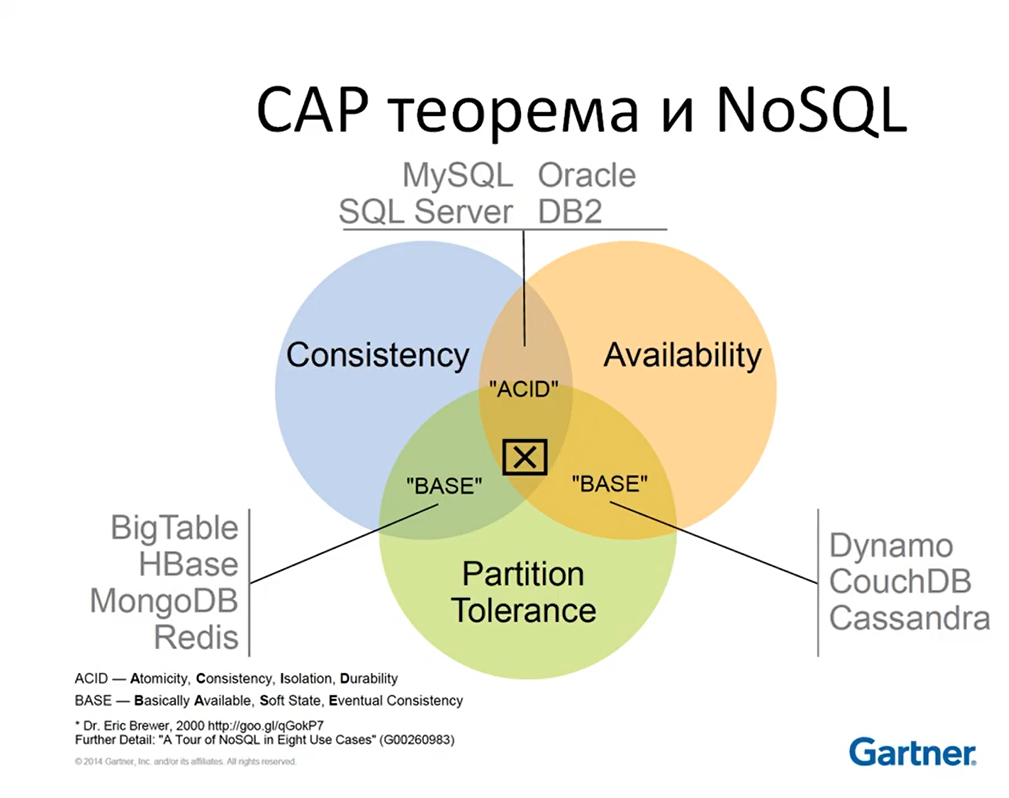
\includegraphics[width = .7\linewidth]{img3}
    \caption{Пример}
\end{figure}

\subsubsection{Хранилище ключ-значение}
\begin{itemize}
    \item Использует принцип асоциативного массива
    \item Базовые операции:
    \begin{itemize}
        \item \textbf{INSERT (ключ, значение)
        \item FIND (ключ)
        \item REMOVE (ключ)}
    \end{itemize}
    \item Как правило реализует класс AP.
\end{itemize}

\newpage

\subsubsection{Документоориентированные БД}

\begin{itemize}
    \item Хранение иерархических структур данных (документов)
    \item Использование стандортных нотаций для описания структур документов: XML, JSON.
    \item Документы индентифицируются ключами
    \item Есть CP и AP Реализации.
\end{itemize}

\begin{figure}[H]
    \centering
    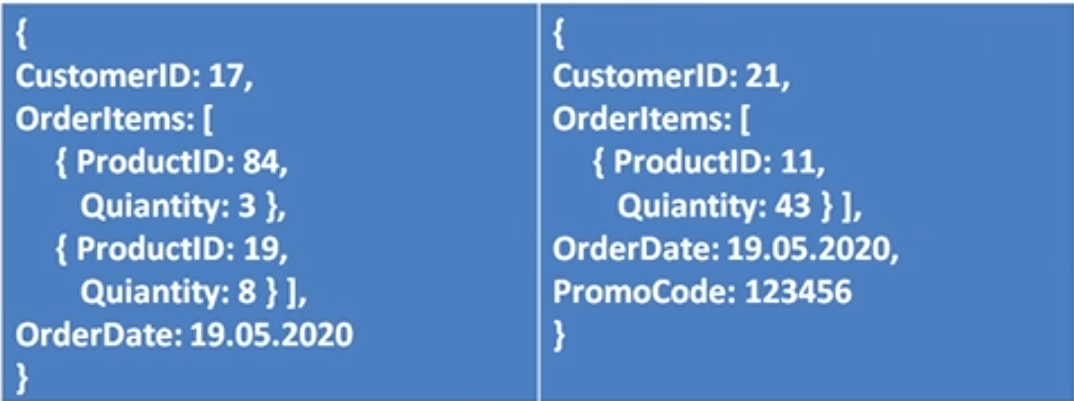
\includegraphics[width = .7\linewidth]{img0}
    \caption{Пример}
\end{figure}
 
 \subsubsection{Колоночные БД}

 \begin{itemize}
     \item Хранение всей таблицы, но с физическим расположением не записей построчно, а атрибутов по колонкам (может использоваться и с реляционной схемой).
     \item Хранение нескольких таблиц с дублированием ключевого атрибута (в пределе переходим к "ключ-значение").
     \item Как правило CA, но могут быть и CP.
 \end{itemize}
 
 \begin{figure}[H]
    \centering
    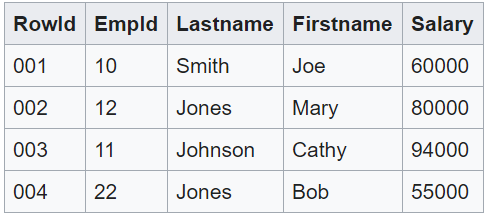
\includegraphics[width = .7\linewidth]{img2}
    \caption{Пример}
\end{figure}
 
 \subsubsection{Графовые БД}
 
 \begin{itemize}
     \item Два типа хранимых объектов: узлы и дуги. У каждого могут быть свои атрибуты.
     \item Удобно для хранения соц. сетей, онтологий и баз знаний.
 \end{itemize}
 
\begin{figure}[H]
    \centering
    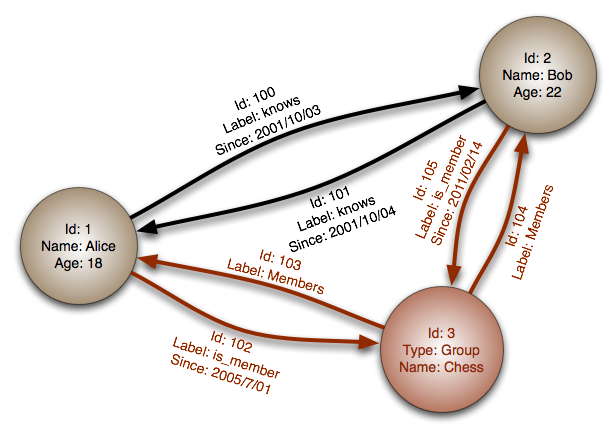
\includegraphics[width = .7\linewidth]{img1}
    \caption{Пример}
\end{figure}
 

\end{document}
